% Tutorial set: 05
% Source: tute5.pdf, PDF pp. 1--2, Questions 1--2
% Reference: tute5_ans.pdf, PDF pp. 2--18 and 20--33
% Session date: 2026-09-16
% Status: Reference experiments explained; training not independently rerun.

\exercisegroup{SC4001-TUT05}{Tutorial 05：Model Selection、Overfitting 与 Regularization}
\label{tutorial:SC4001-TUT05}

\exercisemeta
  {SC4001-TUT05}
  {2026-09-16}
  {\texttt{tute5.pdf} pp.~1--2，Q1--Q2；\texttt{tute5\_ans.pdf} pp.~2--18、20--33}
  {参考实验已讲解；题意、方法与图表已核对，未重新训练}
  {已请求整理笔记（2026-09-16）}

本组是 programming/experiment tutorial（编程与实验习题）。以下数值和曲线均来自参考答案，不是本次独立复现的结果；流程中的严谨性补充另行说明。

\exercisequestion{SC4001-TUT05-Q01}{Function Regression：三种模型选择方法}
\nopagebreak[4]

\textbf{对应讲义：}
\relatedtopic{SC4001-L05-T01}{参数、超参数与误差}；
\relatedtopic{SC4001-L05-T02}{随机重复划分}；
\relatedtopic{SC4001-L05-T03}{交叉验证}；
\relatedtopic{SC4001-L05-T04}{三路划分与数据泄漏}

\subsubsection*{题目与统一设置}

在 $[-1,1]^2$ 上取等间距 $10\times10$ 网格，共 $100$ 个样本，拟合
\[
  y=\sin(\pi x_1)\cos(2\pi x_2).
\]
网络只有\textbf{一层隐藏层}和一个 linear output neuron（线性输出神经元）；候选隐藏宽度
$m\in\{2,4,6,8,10\}$，学习率 $\alpha=0.05$，用 early stopping（早停）结束训练。分别采用
(a) $70{:}30$ random subsampling（随机重复划分）、
(b) five-fold cross-validation（五折交叉验证）、
(c) 近似等分的 train/validation/test（训练/验证/测试）三路划分；每种流程做 $10$ 次实验，选择宽度并估计误差。

\begin{workedsolution}
\nopagebreak[4]
参考实现（答案 pp.~4--8）采用 $2\to m\to1$ 的 sigmoid hidden layer（Sigmoid 隐藏层）、线性输出、SGD 和 MSE。这里的 perceptron 不表示用不可导的硬阈值训练；输出也不能再加 sigmoid，因为目标值可以为负。

\textbf{先理解 held-out error（留出误差）。}
令 $H$ 是没有直接参与该模型梯度更新的留出样本集合，则
\[
  E_H(m)=\frac{1}{|H|}\sum_{(\bm x_i,y_i)\in H}
  \bigl(f_{\bm\theta_m}(\bm x_i)-y_i\bigr)^2.
\]
这是\emph{整个留出集合的平均误差}，不是 training error（训练误差），也通常不是只看一个 validation sample（验证样本）。若用 $H$ 选择宽度或停止 epoch，它就承担 validation set（验证集）的角色；即使变量名叫 \texttt{test}，也不再是 untouched test set（未参与选择的测试集）。

\subsubsection*{(a) Random Subsampling：先对每个宽度求平均，再选宽度}

第 $r$ 次实验重新随机分出 $70$ 个 training samples 和 $30$ 个 held-out samples；在该次相同划分上，分别训练五个候选宽度。记其留出 MSE 为 $E_{r,m}$，则
\[
  \overline E_m=\frac{1}{10}\sum_{r=1}^{10}E_{r,m},
  \qquad m^*=\arg\min_{m\in\{2,4,6,8,10\}}\overline E_m.
\]
因此共比较 $10\times5=50$ 次候选训练，而不是每次只挑一个宽度。重复划分可减轻对某一次 split（划分）的依赖，但不同实验的留出集合可以重叠。

参考答案 p.~11 的最低平均误差出现在 $\boxed{m=4}$，从图读取约为 $0.2376$。
原题要求 train:test $=70{:}30$；答案 p.~10 的文字却写成 $30{:}70$，此处按原题记录，不能仅凭该页确认实际运行时的比例。

\subsubsection*{(b) Five-fold Cross-validation：轮流留一折验证}

把 $100$ 个样本分为五个互不重叠的 folds（折），每折 $20$ 个。固定宽度 $m$，第 $k$ 次用其他四折的 $80$ 个样本训练，用第 $k$ 折验证；每折重新初始化模型，不能沿用上一折的参数。
\[
  E^{\mathrm{CV}}_{r,m}=\frac15\sum_{k=1}^{5}E_{r,k,m},
  \qquad
  \overline E^{\mathrm{CV}}_m=\frac1{10}\sum_{r=1}^{10}E^{\mathrm{CV}}_{r,m}.
\]
在第 $r$ 次五折划分内，每个样本恰好用于一次验证、四次训练；再重复整个五折流程 $10$ 次，按 $\overline E^{\mathrm{CV}}_m$ 选宽度。候选训练次数为 $10\times5\times5=250$。

答案 p.~14 同样选出 $\boxed{m=4}$，最低平均 CV error（交叉验证误差）从图读取约为 $0.2494$。CV 可用于比较候选模型，但\textbf{选中模型的最小 CV error 不自动成为独立、无选择偏差的最终测试误差}。

\subsubsection*{(c) Three-way Split：训练、选择与最终评价分工}

每次将数据近似等分，例如 $33/33/34$；$100$ 不能精确三等分。三个集合分别负责：
\begin{enumerate}
  \item \textbf{Training set：}对每个候选宽度拟合 weights/biases（权重/偏置）。
  \item \textbf{Validation set：}比较候选宽度，并决定 early stopping。
  \item \textbf{Test set：}选择规则确定后，用于最后评价，不反过来修改模型。
\end{enumerate}
参考流程还将 train 与 validation 合并，对选定宽度重新训练后评价 test。严谨性补充：合并后，原 validation 已变为 training data；若仍需 early stopping，必须另留内部验证集，或使用此前确定的训练 epoch 数，不能改用 test 决定停止。

答案 p.~18 列出的十次获选宽度为
\[
  8,\ 8,\ 2,\ 6,\ 2,\ 2,\ 4,\ 2,\ 4,\ 4.
\]
其中 $2$ 出现四次，答案按 mode（众数）总结为 $\boxed{m=2}$，并报告合并 train/validation 后的平均 MSE 为 $0.215$。该页的 ``hidden layers = 2'' 应理解为\textbf{隐藏神经元数为 2}，不是两层隐藏层。

\textbf{结果应怎样理解？}
(a)(b) 是先对每个宽度平均误差再取最小值；(c) 参考页则总结每次获选宽度的众数。这些数值还来自不同的数据划分与评价流程，不能仅凭 $0.215<0.2376<0.2494$ 就断言三路划分训练出了普遍更好的模型，也不能把某次实验的最佳宽度视为理论最优。

\textbf{Early stopping 的正确评价口径。}
监控 validation loss（验证损失），保存并在结束时恢复最佳 validation checkpoint（验证检查点）；最后一个 epoch 不一定最好。答案 p.~8 将 \texttt{test\_loss} 传入 stopper，因此该集合已用于模型选择，不能同时宣称它提供完全独立的测试评价。
\end{workedsolution}

\exercisequestion{SC4001-TUT05-Q02}{CIFAR-10：Network Size、Dropout、Weight Decay 与 Grid Search}
\nopagebreak[4]

\textbf{对应讲义：}
\relatedtopic{SC4001-L05-T05}{Model Complexity、Underfitting 与 Overfitting}；\par\noindent
\relatedtopic{SC4001-L05-T06}{Early Stopping、Regularization 与 Dropout}；\par\noindent
\relatedtopic{SC4001-L05-T04}{Three-way Split 与 Data Leakage}

\subsubsection*{题目与统一设置}

CIFAR-10 共 $60\,000$ 张 $32\times32$ 彩色图像、$10$ 类，每类 $6\,000$ 张；官方划分为 $50\,000$ 张 training images 与 $10\,000$ 张 test images，从 \texttt{torchvision.datasets.CIFAR10} 读取。
全部实验使用 Adam、学习率 $0.001$、batch size $256$、early-stopping patience $10$。原题的 ``Adams'' 指 Adam。

\begin{enumerate}[label=(\alph*)]
  \item 比较三个各含三层 hidden ReLU layers（隐藏 ReLU 层）的全连接网络：每层宽度分别为 $50$、$100$、$400$；绘制 train/test cross-entropy（交叉熵）随 epoch 的曲线，讨论欠拟合与过拟合。
  \item 在大网络上分别搜索 weight decay（权重衰减）
    $\beta\in\{0.0001,0.001,0.01\}$ 和 dropout rate（丢弃率）
    $p\in\{0.1,0.2,0.4\}$，选择最佳设置并画学习曲线。
  \item 用 Ray Tune 联合搜索
    $\{0.0001,0.001,0.005,0.01\}\times\{0.1,0.2,0.3,0.4\}$
    中的 $(\beta,p)$，绘制最佳组合的学习曲线。
\end{enumerate}

\begin{workedsolution}
\nopagebreak[4]
\textbf{架构与 loss。}
Flatten（展平）后输入维度为 $32\times32\times3=3072$，网络为
\[
  3072\xrightarrow{\mathrm{ReLU}}h
  \xrightarrow{\mathrm{ReLU}}h
  \xrightarrow{\mathrm{ReLU}}h
  \xrightarrow{\mathrm{linear}}10,
  \qquad h\in\{50,100,400\}.
\]
每条箭头包含一层全连接变换；前三层随后使用 ReLU。最终十维输出是 raw logits（原始逻辑值），直接送入 \texttt{CrossEntropyLoss}，无需先做 Softmax。

\textbf{数据分工的严谨性补充。}
原题用 train/test 命名，参考答案 pp.~23、30 也用 \texttt{test\_loss} 做早停和调参；因此这些曲线中的留出数据实际上参与了验证。若要求独立的最终评价，应从官方 $50\,000$ 张训练图像中再划出 validation，把官方 $10\,000$ 张 test 留到最后。原题没有规定这一额外划分的比例。

\subsubsection*{(a) 改变 Network Size：看两条曲线，不只看差距}

图~\ref{fig:sc4001-tut05-size} 中蓝、绿、红分别为 $50$、$100$、$400$ 宽度；虚线为 train，实线为原图标注的 validation。
\begin{itemize}
  \item \textbf{Small network：}训练与留出损失均较高，符合 underfitting（欠拟合）的典型表现。
  \item \textbf{Medium network：}留出损失较低，参考答案认为其复杂度较合适。
  \item \textbf{Large network：}留出损失较早停滞，参考答案将其解释为 overfitting（过拟合）。不过图中的大网络训练损失并不是最低，不能据此声称“大网络一定把训练集拟合得最好”；仅凭这组曲线也不能排除优化不足等因素。
\end{itemize}

\begin{figure}[H]
  \centering
  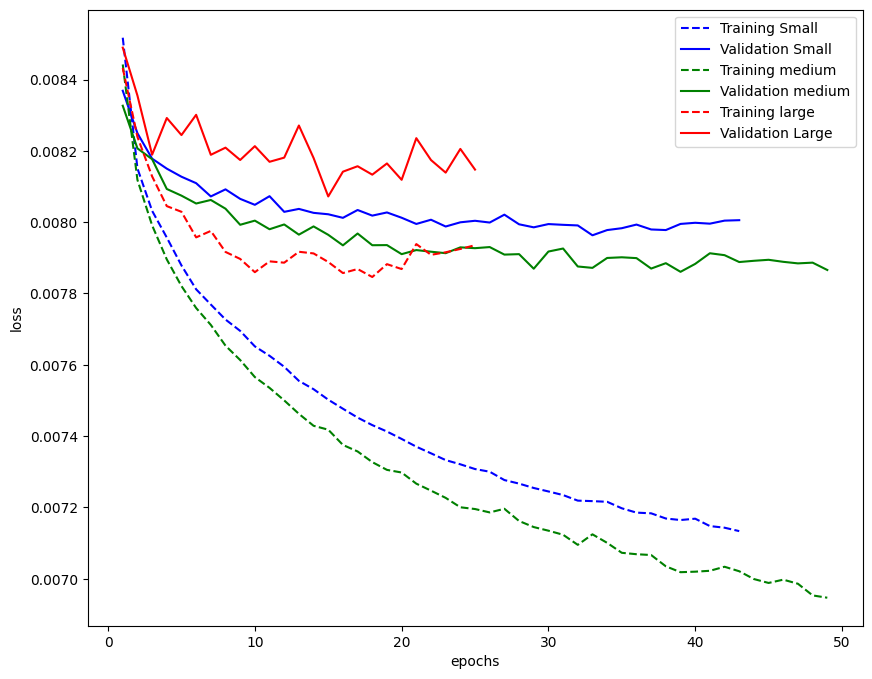
\includegraphics[width=0.82\textwidth]{figures/source/tutorial-05-network-size.png}
  \caption{不同网络宽度的原始参考曲线。来源：SC4001 \texttt{tute5\_ans.pdf} p.~24，仅提取图表；轴刻度与图例保留原样，非本次训练结果。}
  \label{fig:sc4001-tut05-size}
\end{figure}

\keyidea{训练损失下降而留出损失上升是过拟合的重要信号；选择模型主要看留出损失，而不是只追求更低的训练损失或更小的 train/validation gap（训练/验证差距）。}

\subsubsection*{(b) 分别使用 Dropout 与 Weight Decay}

\textbf{Dropout：}参考网络在三个隐藏层的 ReLU 后各加一层 dropout，输出层不加。训练时每个隐藏 activation（激活值）以概率 $p$ 被置零；$p=0.4$ 表示丢弃 $40\%$，不是保留 $40\%$。推理或验证时应关闭随机丢弃；常用 inverted dropout（反向缩放的 dropout）在训练时将保留激活除以 $1-p$，保持条件期望不变。

答案 p.~27 在给定候选中选择 $\boxed{p=0.4}$。图~\ref{fig:sc4001-tut05-dropout} 还绘制了 $p=0$ 的基线：无 dropout 时训练损失持续下降，而留出损失后来回升；合适的 dropout 虽让训练更难，却能降低留出损失。启用与关闭 dropout 时的损失是在不同条件下计算，不能机械地把二者差距都解释为泛化差距。

\begin{figure}[H]
  \centering
  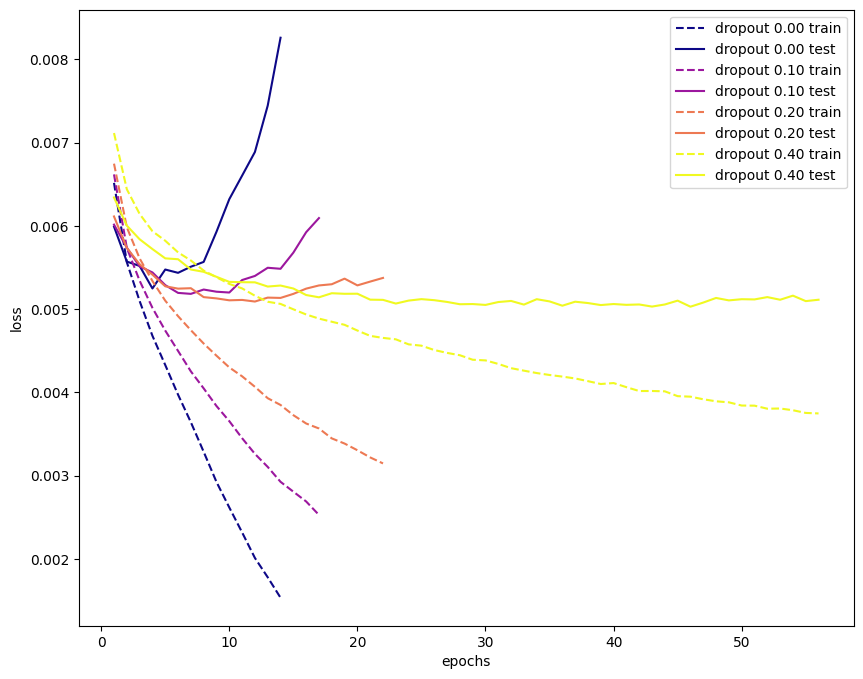
\includegraphics[width=0.82\textwidth]{figures/source/tutorial-05-dropout.png}
  \caption{单独改变 dropout rate 的参考曲线。来源：SC4001 \texttt{tute5\_ans.pdf} p.~27；图例中的虚线为训练曲线，实线为留出曲线，标签保留原样。}
  \label{fig:sc4001-tut05-dropout}
\end{figure}

\textbf{Weight decay：}限制权重过大，以控制模型的有效复杂度。可用 L2-regularized objective（L2 正则化目标）理解这一动机：
\[
  J_{\mathrm{reg}}(\bm\theta)
  =J_{\mathrm{data}}(\bm\theta)+\frac\beta2\lVert\bm W\rVert_2^2.
\]
这里是原理示意；具体哪些参数被惩罚及更新形式由实现决定，不应把所有优化器中的 weight decay 都视为完全相同的操作。

答案 p.~28 在候选中选择 $\boxed{\beta=0.001}$。图~\ref{fig:sc4001-tut05-decay} 也包含 $\beta=0$ 的基线。$\beta=0.01$ 虽使两条曲线靠近，却有更高的留出损失，说明 regularization（正则化）过强也可能导致欠拟合；\textbf{差距更小不等于模型更好}。

\begin{figure}[H]
  \centering
  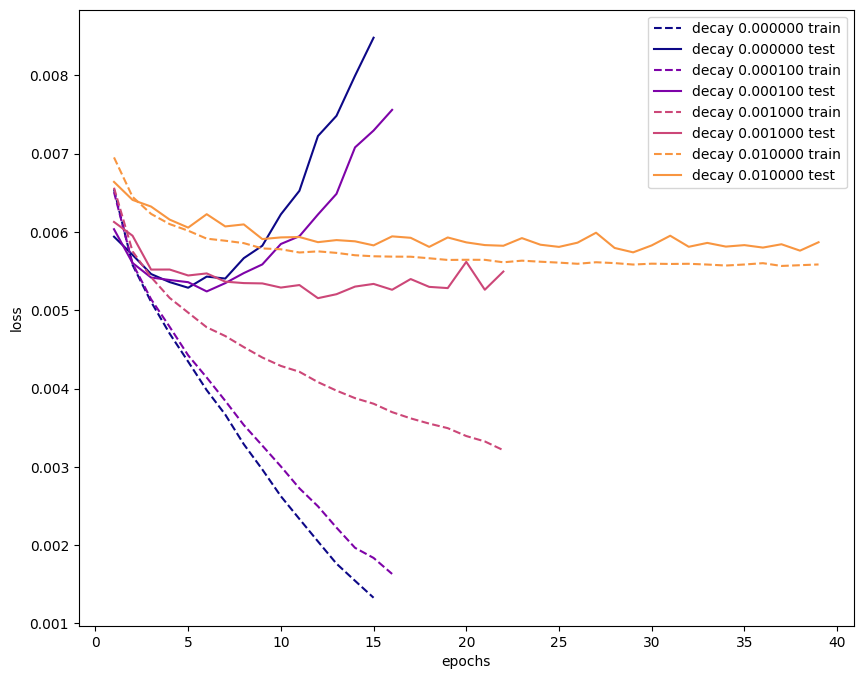
\includegraphics[width=0.82\textwidth]{figures/source/tutorial-05-weight-decay.png}
  \caption{单独改变 weight decay 的参考曲线。来源：SC4001 \texttt{tute5\_ans.pdf} p.~28；不能只按虚线与实线的距离选择正则化强度。}
  \label{fig:sc4001-tut05-decay}
\end{figure}

\subsubsection*{(c) Joint Grid Search：最优组合不等于单独最优值的拼接}

两个参数各四个候选，因此有 $4\times4=16$ 个 configurations（配置）。每个配置都应独立初始化模型与 optimizer（优化器），训练后按同一 validation criterion（验证标准）比较。Ray Tune 负责组织 trials（试验）与记录结果，并不代替 Adam 更新网络权重。

图~\ref{fig:sc4001-tut05-grid} 左侧是 loss，颜色越暗越好；右侧是 accuracy（准确率），颜色越亮越好。横轴为 dropout，纵轴为 weight decay。参考答案 pp.~31--32 的最佳组合为
\[
  \boxed{\beta=0.0001,\qquad p=0.4}.
\]
单独使用 weight decay 时选 $0.001$，联合时改为 $0.0001$，并不矛盾：dropout 已提供一部分正则化，两个超参数相互影响，不能把单参数搜索的最优值直接拼起来。

\begin{figure}[H]
  \centering
  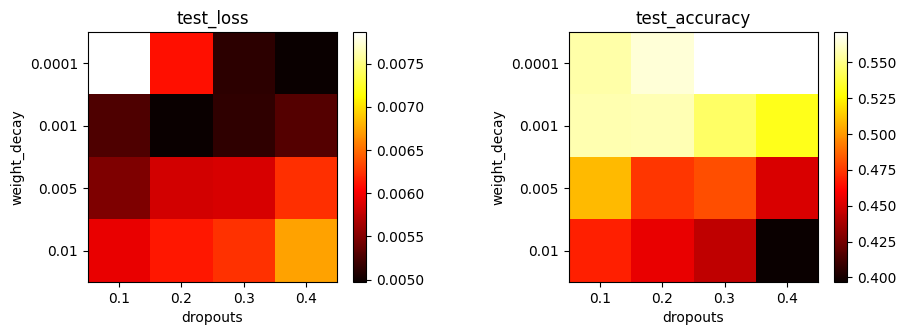
\includegraphics[width=0.98\textwidth]{figures/source/tutorial-05-grid-search.png}
  \caption{联合 grid search（网格搜索）的参考热力图。来源：SC4001 \texttt{tute5\_ans.pdf} p.~32。原图将指标标为 test；结合 p.~30 的选择代码，这些指标参与了调参，应按验证结果理解。}
  \label{fig:sc4001-tut05-grid}
\end{figure}

\textbf{参考实现与图表的边界。}
答案 p.~26 的类定义默认 \texttt{hidden\_size=500}，但题目要求大网络宽度 $400$，实现时应显式按原题设置。
\verify{幻灯片未给出该类的实际调用参数，不能确认图中网络是否覆盖了这一默认值。}
另一个口径差异是 p.~33 的汇总曲线把单独 weight decay 标为 $0.0100$，与 p.~28 报告的最佳值 $0.001$ 不一致；因此不能把该曲线描述成“两个单独最优方法与联合最优方法的公平比较”。

本题应掌握的是\textbf{候选配置只用验证集选择，最终测试集不参与选择}，以及\textbf{按留出损失判断复杂度与正则化强度}。参考最优参数只适用于课件所示实验；当前没有完整训练日志与运行配置，未将它们当作可重复保证的结论。
\end{workedsolution}
